\ylDisplay{Varjud} % Ülesande nimi
{Jaak Kikas} % Autor
{piirkonnavoor} % Voor
{2007} % Aasta
{G 6} % Ülesande nr.
{4} % Raskustase
{
% Teema: Geomeetriline-optika
\ifStatement
Läbipaistmatut kera valgustab kerakujuline valgusallikas. Joonisele on kantud läbipaistmatu kera poolt tekitatud täis- ja poolvarju koonuste lõiked joonise tasandiga (kera keskpunkt asub samas tasandis). Konstrueerige valgusallika lõige joonise tasandiga. Valgusallika keskpunkt asetseb samuti joonise tasandis.

\begin{center}
	
\includegraphics[height=0.8\textheight]{2007-v2g-06-yl}
\end{center}
\fi


\ifHint
Nii täis- kui poolvarjude piirjoonte pikendused on valgusallika puutujad.
\fi


\ifSolution
Kanname joonisele varjukoonuste piirjoonte pikendused (sirged 1-4). Valgusallikaks oleva kera lõikejoon joonise tasandiga on ringjoon, mille puutujateks on kõik need sirged. Selle keskpunkti leidmiseks konstrueerime sirgete 1-3 ja 2-4 poolt moodustatud nurkade poolitajad (punktiirjooned joonisel), nende lõikepunkt 0 on otsitava ringjoone keskpunktiks. Ringi raadiuse leidmiseks konstrueerime punktist 0 mõnele sirgetest 1-4 keskristssirge.

\begin{center}
	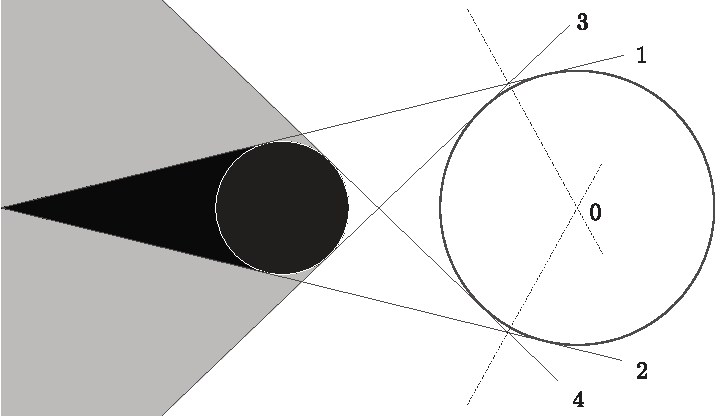
\includegraphics[width=\textwidth]{2007-v2g-06-lah}
\end{center}
\fi
}